\documentclass[12pt,A4]{extarticle}	

\usepackage{amsfonts}
\usepackage{amsmath}
\usepackage{amssymb}
\usepackage{graphicx,wrapfig,lipsum}

\newcommand{\lectureTitle}{Symmetrische Verschlüsselungsverfahren [WIP]}
\newcommand{\semester}{Sommersemester 2023}

\newcommand{\titleSize}{\LARGE}

\usepackage[a4paper,left=0.9cm,right=1cm,top=1.37cm,bottom=2.5cm]{geometry}
\usepackage[utf8]{inputenc}
\usepackage{xifthen}
\usepackage{cmbright}
\usepackage{fontawesome}
\usepackage[T1]{fontenc}
\usepackage{lastpage,lipsum}
\usepackage{hyperref}
\usepackage{transparent}
\usepackage{color}
\usepackage{fancyhdr}

\renewcommand*\familydefault{\sfdefault}
\setlength{\parindent}{0mm}

\definecolor{headerBg}{RGB}{11, 67, 158}
\definecolor{headerGrayColor}{RGB}{210, 210, 210}

\newcommand{\printTitle}{\textcolor{white}{\lectureTitle}\normalsize}
\newcommand{\printSubtitle}{
  \ifdefined\lectureSubtitle
    \textcolor{white}{\small{\lectureSubtitle}}\\
  \fi
}

\fancyhf{}
\pagestyle{fancy}
\fancyhead[C]{
  \fcolorbox{headerBg}{headerBg}{
    \hspace{0.6cm}\begin{minipage}[c][50pt][c]{\paperwidth}
      \begin{minipage}[c]{.7\textwidth}
        \ifdefined\titleSize
          \titleSize \printTitle\\
        \else
          \huge\printTitle\\
        \fi
        \printSubtitle
        \textcolor{headerGrayColor}{\small{\semester}}
      \end{minipage}%
      \begin{minipage}[c]{.2\textwidth}
        \raggedleft
        \textcolor{white}{
          \small{\href{mailto:mail@nilslambertz.de}{\textcolor{white}{\faicon{envelope}} mail@nilslambertz.de}}\\
          \href{https://github.com/nilslambertz/kit-zusammenfassungen}{\textcolor{white}{\faicon{github}} \small{nilslambertz}}}
      \end{minipage}
    \end{minipage}}
}
\renewcommand{\headrulewidth}{0pt}
\setlength{\headheight}{40pt}

\newlength{\oddmarginwidth}
\setlength{\oddmarginwidth}{1in+\hoffset+\oddsidemargin}
\newlength{\evenmarginwidth}
\setlength{\evenmarginwidth}{\evensidemargin+1in}
\fancyhfoffset[LO,RE]{\oddmarginwidth}
\fancyhfoffset[LE,RO]{\evenmarginwidth}
\cfoot{\thepage\ $/$ \pageref*{LastPage}}

\definecolor{highlightColor}{RGB}{66, 135, 245}
\newcommand{\highlight}[1]{\textcolor{highlightColor}{\textbf{#1}}}

\def\contentsname{\empty}

\begin{document}

\disclaimer

\tableofcontents
\clearpage

\section{Einführung}
\subsection{Ausgangspunkte für Angriffe}
Angriffe können nach den zur Verfügung stehenden Informationen unterteilt werden:
\begin{itemize}
  \item{\highlight{Ciphertext-Only-Attack}: Nur das \textit{Chiffre}, also die verschlüsselte Nachricht, ist bekannt}
  \item{\highlight{Known-Plaintext-Attack}: Es gibt bekannte Klartext-Chiffre-Paare. Hilfreich sind bekannte Anfangs- und Endphrasen, die in mehreren Nachrichten vorkommen.}
  \item{\highlight{Chosen-Plaintext-Attack}: Es besteht die Möglichkeit, beliebige Texte zu verschlüsseln und somit Klartext-Chiffre-Paare zu erzeugen.}
\end{itemize}

\subsection{Angriffsarten}
\begin{itemize}
  \item{Brute-Force (z.B. alle Schlüssel ausprobieren)}
  \item{Statistische Methoden (z.B. Häufigkeitsanalysen von Buchstaben)}
  \item{Strukturelle Angriffe (z.B. Lineare Kryptoanalyse)}
\end{itemize}

\subsection{Historische Verschlüsselungsverfahren}
Historisch wurden zur Verschlüsselung zwei grundlegende Operationen verwendet:
\begin{itemize}
  \item{\highlight{Substitution}}
  \item{\highlight{Permutation}}
\end{itemize}
Alleine sind beide Verfahren meistens nicht sicher, jedoch verwenden moderne Verschlüsselungsverfahren eine Kombination beider Operationen.

\section{Blockchiffren}
\subsection{Definitionen}
\subsubsection{Definition: Blockchiffre}
Gegeben seien zwei endliche Alphabete $A, B$ und $n, m \in \mathbb{N}$ sowie ein Schlüsselraum $\mathcal{K}$. Eine \highlight{Blockchiffre} ist gegeben durch eine Familie von injektiven Abbildungen $f_k: A^n \rightarrow B^m$ mit $k \in \mathcal{K}$. In der Regel gilt $A = B = \{0, 1\}$ und $n = m$.

\subsubsection{Anforderungen an Blockchiffren}
\begin{itemize}
  \item{Gegeben den Schlüssel $k$ müssen sowohl $f_k$ als auch $f^{-1}_k$ \textbf{effizient} berechenbar sein}
  \item{Ein Angreifer soll nicht zwischen einer \textit{zufälligen Abbildung} und der Blockchiffre mit \textit{zufälligem Schlüssel} unterscheiden können}
\end{itemize}

\subsubsection{Definition: Ideal Cipher}
Eine \highlight{Ideal Cipher} (IC) ist eine (Über-)Idealisierung einer Blockchiffre. Jedem Schlüssel $k \in \{0, 1\}^\lambda$ ist eine vollkommen zufällige Permutation $P_k: \{0, 1\}^n \rightarrow \{0, 1\}^n$ zugeordnet (hierbei sind $\lambda$ und $n$ Sicherheitsparameter) und per Orakelzugriff kann jede Maschine im Modell die Funktionen $P_k$ und $P^{-1}_k$ auswerten. Die Existenz einer solchen IC wird zur Vereinfachung von Beweisen angenommen, man spricht dann von dem \textbf{Ideal-Cipher-Modell}.

\subsubsection{Anforderungen an Ideal Cipher}
\begin{itemize}
  \item{Alle Parteien können über Orakelzugriff $P_k$ und $P^{-1}_k$ auswerten}
  \item{Ideal Cipher liefert zu jedem Paar $(k, m)$ ein $c$ ``zufällig'' gewählt}
  \item{Ideal Cipher liefert zu jedem Paar $(k, c)$ ein $m$ ``zufällig'' gewählt}
  \item{Orakel muss jede Ausgabe speichern, damit für gleiche Nachrichten immer das gleiche Chiffre zurückgegeben wird (nicht parallelisierbar)}
\end{itemize}

\subsection{DES (Data Encryption Standard)}
Der \textbf{Data Encryption Standard} ist eine Blockchiffre mit Schlüssellänge $k = 56$ und Blocklänge $n = 64$, die Verschlüsselungsfunktion ist also $\{0, 1\}^k \times \{0, 1\}^n \rightarrow \{0, 1\}^n$. Er besteht aus einer \textbf{Feistel-Struktur} mit 16 Runden und wurden aufgrund der kurzen Schlüssellänge \textbf{gebrochen}.


\begin{wrapfigure}{r}{9cm}
  \begin{centering}
    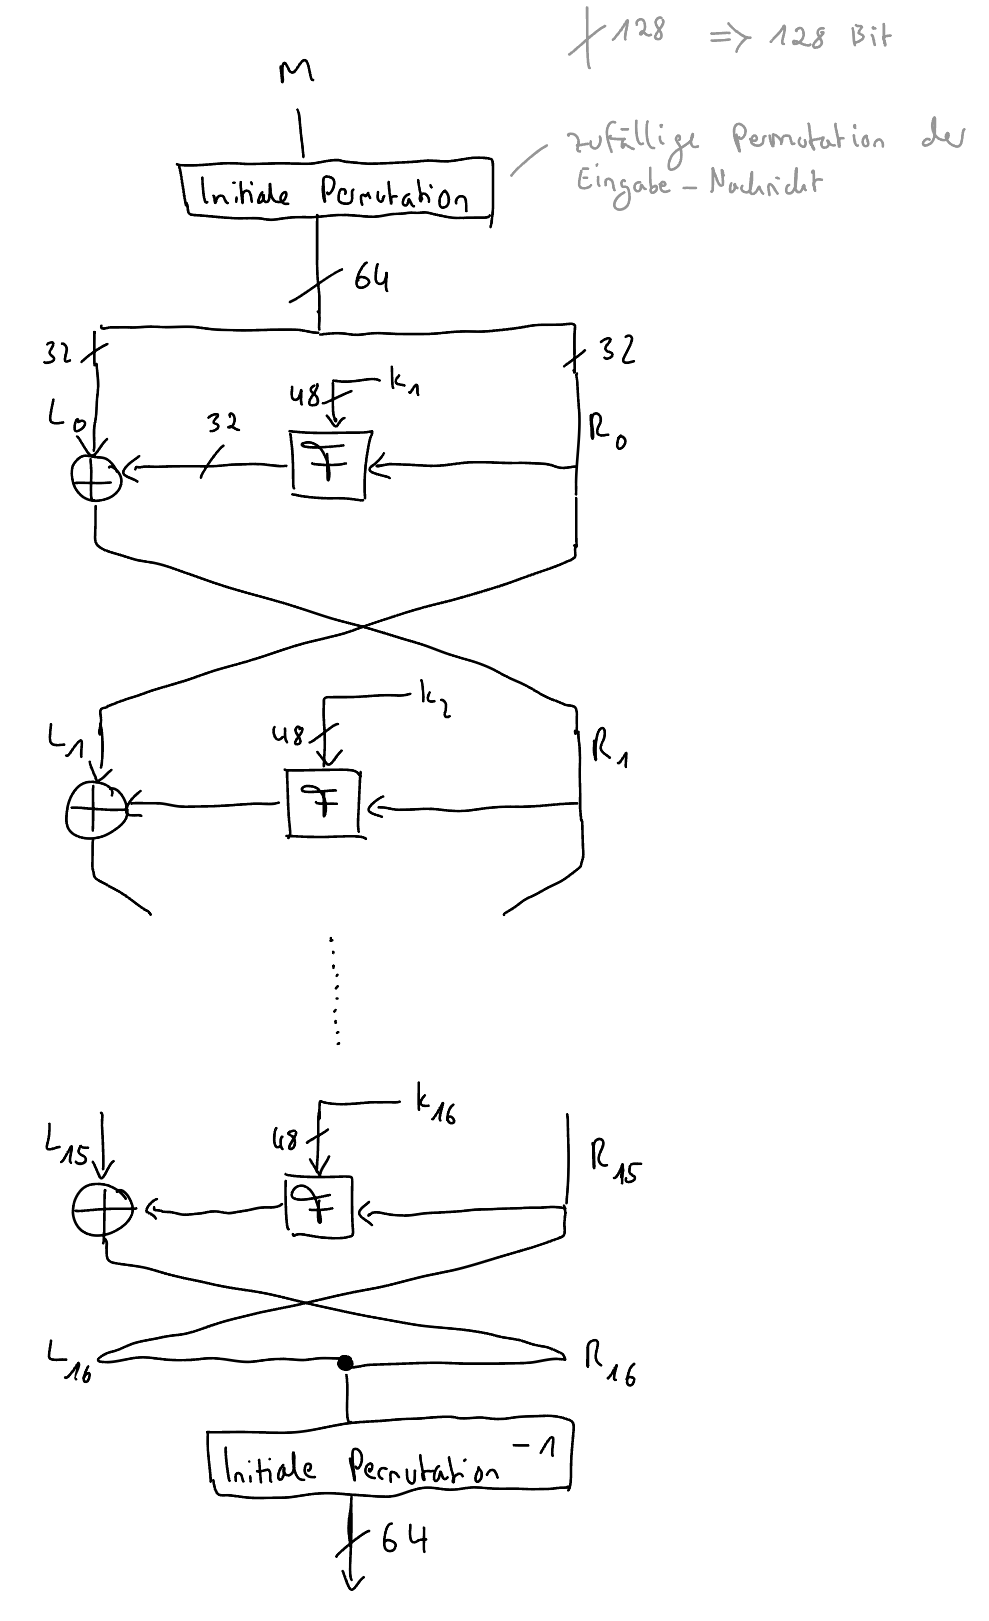
\includegraphics[width=9cm]{images/des_struktur.png}
  \end{centering}
  \caption{DES-Verschlüsselungsalgorithmus}
\end{wrapfigure}
\subsubsection{Beispiel für Encryption-Schritt}
$L_1 = R_0$\\
$R_1 = L_0 \oplus F_{k_1}(R_0)$\par
$L_{16} = R_{15}$\\
$R_{16} = L_{15} \oplus F_{k_{16}}(R_{15})$\par

\subsubsection{Beispiel für Decryption-Schritt}
$R_{15} = L_{16}$
\begin{flalign*}
  L_{15} & = R_{16} \oplus F_{k_{16}}(R_{15}) & \\
         & = R_{16} \oplus F_{k_{16}}(L_{16})
\end{flalign*}

\end{document}